\section{Where the diffusion model wins}
\label{sec:wins}

The diffusion model is faster than AR at any output length above the
crossover $L^{*} = \crossoverL$ tokens. The advantage grows with output
length because AR pays per token while DG pays per canvas.

Table~\ref{tab:niche} shows the comparison at the quality-comparable pair
(\ARoneb\ vs \DG). AR cells are \emph{forced} ($\texttt{min\_tokens} = L$);
the unforced row shows AR-1.5B at its natural output length of 138 tokens.

\begin{table}[h]
\centering
\caption{Latency at comparable quality (AR-1.5B F1 0.868 vs DG 0.852;
within the 0.016 margin). AR-1.5B vs DG-26B-A4B, batch-1, BGL.
$n{=}100$--$300$.}
\label{tab:niche}
\begin{tabular}{@{}lrrrr@{}}
\toprule
$L_{\mathrm{out}}$ & AR-1.5B forced (ms) & AR-1.5B unforced & DG (ms) & DG advantage \\
\midrule
138 (natural) & --- & 665.7 & \dgTwoFive{} & $1.8\times$ \\
256  & \arOneFiveTwoFive{} & --- & \dgTwoFive{}   & $2.7\times$ \\
512  & \arOneFiveFiveOne{} & --- & \dgFiveOne{}   & $4.0\times$ \\
1024 & \arOneFiveTenTwoFour{} & --- & \dgTenTwoFour{} & $5.4\times$ \\
\bottomrule
\end{tabular}
\end{table}

\paragraph{The real advantage is $1.8\times$.}

Even unforced --- at AR-1.5B's natural output length of 138 tokens --- DG
completes in \dgTwoFive\,ms against AR's 665.7\,ms. The $5.4\times$
headline at $L{=}1024$ is inflated by forcing: the parser
(first-object-wins) discards the rambled continuation past the first JSON
object, so the AR arm is charged \arOneFiveTenTwoFour\,ms for output the
scorer deletes. The forced comparison is an upper bound on AR cost, not a
measurement of it. Appendix~\ref{app:forced} shows analytically that the
advantage holds at naturally-long output (multi-record extraction) without
forcing.

\begin{figure}[t]
\centering
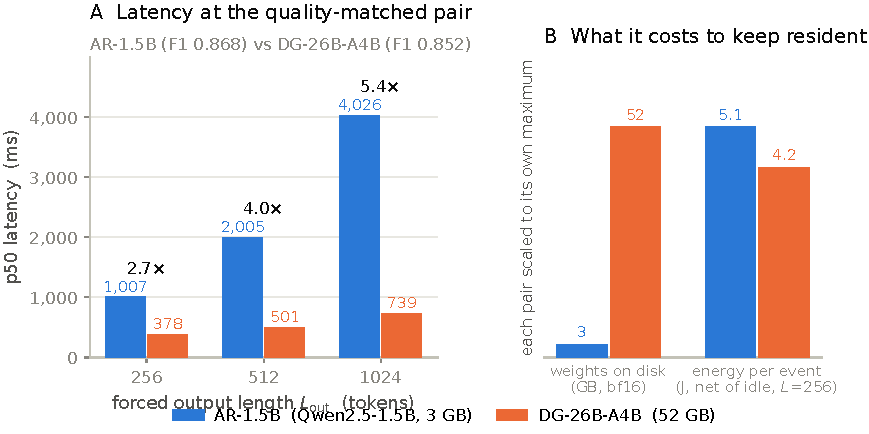
\includegraphics[width=\linewidth]{figures/fig9_deployment.pdf}
\caption{The quality-comparable deployment pair (BGL, $n{=}100$,
$K{=}8$). \textbf{A:} at forced output lengths the diffusion model's
advantage is real and grows, because the AR model rambles well past its
natural length ($\sim$138 tokens). \textbf{B:} the standing cost of
keeping each model resident. Energy per event is net of idle draw; the
two energy runs recorded different idle baselines (52.6\,W and 58.6\,W),
so treat the energy comparison as indicative.}
\label{fig:deploy}
\end{figure}

\paragraph{Energy.}

The diffusion model uses less energy because it is busy for less time.
At the compute-matched pair (\ARthree\ vs \DG):
\begin{align}
\text{compute-matched:} \quad & R_{\mathrm{energy}} =
\frac{\arThreeEnergy}{\dgEnergy} = 5.3 \quad \text{(idle 52.6\,W)} \\
\text{quality-comparable:} \quad & R_{\mathrm{energy}} =
\frac{\arOneFiveEnergy}{\dgEnergy} = 1.2 \quad \text{(idle 58.6\,W)}
\end{align}
The two energy runs had different idle baselines, so the
quality-comparable comparison is indicative.

\paragraph{Graceful degradation.}

Under deadline pressure the diffusion model returns a complete canvas at
lower quality, while the AR model returns a truncated record that fails
schema validation. At a p99 budget of 400\,ms, dropping $K$ from 8 to 4
meets it at \kFourPninetynine\,ms p99 with F1 falling from \kEightFone\
to \kFourFone.
